\documentclass[11pt, oneside]{article}   	% use "amsart" instead of "article" for AMSLaTeX format
\usepackage{geometry}                		% See geometry.pdf to learn the layout options. There are lots.

\geometry{letterpaper}                   		% ... or a4paper or a5paper or ... 
%\geometry{landscape}                		% Activate for rotated page geometry
\usepackage[parfill]{parskip}    			% Activate to begin paragraphs with an empty line rather than an indent
\usepackage{graphicx}				% Use pdf, png, jpg, or eps§ with pdflatex; use eps in DVI mode
								% TeX will automatically convert eps --> pdf in pdflatex
\usepackage{amssymb}

\usepackage{hyperref} 				% you need this package
\usepackage{pifont}					% for \ding

% Make clickable footnote
\newcommand{\hyperfootnote}[1][]{\def\ArgI{{#1}}\hyperfootnoteRelay}
  % relay to new command to make extra optional command possible
\newcommand\hyperfootnoteRelay[2][]{\href{#1#2}{\ArgI}\footnote{\href{#1#2}{#2}}}
  % the first optional argument is now in \ArgI, the second is in #1
  
% Takes at most 3 parameters (see http://www.tex.ac.uk/FAQ-twooptarg.html for info on multiple optional parameters)
% If first parameter isn't given, it's value is '' (empty string in text before footnote reference)
% If second parameter isn't given, it's value is '' (string before visible URL, e.g. 'http://')
% Makes a clickable footnote (alternatively: \url{}) with optional reference in the text as well
% Use 1: \hyperfootnote{www.mywebsite.com}: creates a footnote consisting of a clickable URL
% Use 2: \hyperfootnote[My website]{www.mywebsite.com}: creates a clickable piece of text in the text ('My website') plus a footnote consisting of a clickable URL
% Note: requires the hyperref package.
% Note: use xspace package to add/absorb spaces when necessary (e.g. to avoid a space between the footnote number and a punctuation mark)

% Info on how to define a LaTeX command: https://www.sharelatex.com/learn/Commands

%SetFonts

\title{Identity Agents}
\author{Paul Trevithick, The Mee Foundation}
%\date{}							% Activate to display a given date or no date

\begin{document}
\maketitle

\section{Power Asymmetry}
While the emergence of the internet brought new services and experience to billions of users, a power asymmetry has developed between the digital service providers and their user regarding these users' digital identities and personal data. Providers have accumulated power compared to users who have lost power (control) over their own identities and data. 

This was unintentional from a design point of view. The internet's designers preferred decentralized architectures that push computation and storage to the edge and minimize centralized control wherever possible. However, economic factors, including so-called natural monopolies, preferential attachment network effects, economies of scale, and the relative ease of creating centralized solutions have contributed to  concentrations of power on the provider side. 

Efforts to ``re-decentralize the web"[reference needed], and focus on decentralized, p2p architectures have arisen. [insert references to other, related efforts like ProjectVRM]. This concept of identity agents runs parallel to these trends.

To reinforce our focus on power relationships, we use the term \emph{computational power} to refer to software tools that work (i.e. provide agency) ``on the user's side" for, and \emph{exclusively} on behalf of, the user. We are not talking about whether the average user's phones and laptops have sufficient computational power; they do. We're saying that this raw computational power and storage is not leveraged by tools that push back on app provider's power, and engage digitally and automatically to empower the user to better manage their relationships with providers on terms more beneficial to them. Since our discussion applies equally provider's mobile apps, webapps, and websites, we simply use the term \emph{app} to refer to all of them.

Power asymmetry lies at the root of a diverse set of related symptoms, most of which erode privacy, since privacy and power are highly interrelated concepts\footnote{Consider the title of C. Veliz's recent book, ``Privacy is Power"[cite]}. 
These privacy eroding symptoms include a lack of personal autonomy, a lack of personal agency, and third-party surveillance.

\subsection{Lack of Autonomy}

\begin{quote}
\textbf{au\tiny \ding{108}\normalsize ton\tiny \ding{108}\normalsize o\tiny \ding{108}\normalsize my}: \emph{freedom from external control or influence; independence.}\hyperfootnote[][https://]{languages.oup.com/google-dictionary-en/}
\end{quote}

\emph{Independence}. In the physical world each of us is a separate, independent entity. Each of us has a self that embodies our individuality. We ``bring" that independent selfness to interactions with others, with vendors, etc. while understanding that this independence is not absolute--we are still to some extent dependent on common, shared systems, laws, environments, and so on. The same cannot be said for our life online where Phil Windley has expressed by saying that "we have no \emph{digital embodiment}\footnote{Phil Windley, personal communication, Sepember 2022}."  Online our identities are provided to us by digital service providers (e.g. in the form of a Facebook identity, or an Amazon account). Without them we don't exist. Anyone who has been banned from a platform, or uses a platform that is shut down is sharply reminded that their digital identity exists at the pleasure of that platform. Our provisional existence is the original power asymmetry. Efforts create personal datastores or even more to the point those that strive to provide each of us a \emph{self-sovereign identity}\cite{Preukschat2021} are squarely aimed at addressing this issue--the word ``sovereignty" certainly evokes power.

\emph{Autonomous data}. Our personal data is collected and held by businesses (first-parties) as we interact with their apps, not by us. This pattern \emph{app-held data} is such a common pattern that it's hard to imagine an alternative. Our data is not ``free from external control" by apps, because it is generally stored and managed by them.

Our data is also collected and held by third-parties (e.g. data brokers) with whom we have no interactions at all. In short, it's been said that \hyperfootnote[“everybody has our data … except us.”][https://]{reb00ted.org/personaldata/20210620-who-has-my-personal-data/}. 

An alternative approach is \emph{user-held} data\cite{Jurcys2021}, where your data is held by you in a personal datastore)\footnote{Examples of open-source personal datastores include \url{https://solidproject.org}, Decentralized Web Nodes(DWN). For more about PDSes see \url{https://wikipedia.org/wiki/Personal\_data\_service}}. 

\emph{Lock-in}. As we've just mentioned our online existence is provisional, but beyond that it is also bound to the platform that originated it. Providers hold our data, and even if they are willing to allow us access (e.g. to download a copy), we lack the ability to accept the data stream, a personal datastore to hold it, and the ability to transform it into other formats and schemas so as to be usable in other contexts. Our lack of agency in these areas results in our data being held hostage, i.e. without autonomy. As Tim Berners-Lee has recently said, "We are locked into platforms that hold our data" [need to check and get reference]. 

[No ability to communicate with others peer-to-peer without relying on an intermediary]

\subsection{Lack of agency}

\begin{quote}
\textbf{a\tiny \ding{108}\normalsize gen\tiny \ding{108}\normalsize cy}: \emph{the capacity, condition, or state of acting or of exerting power} \hyperfootnote[][https://]{www.merriam-webster.com/dictionary/agency}
\end{quote}

\emph{Wielding credentials}. In the offline world you can autonomously present you drivers license to a wine seller to prove you exceed the minimum drinking age. The wine seller trusts the issuer of the license, not you. This interaction could be described as ``wielding" a trust credential. By contrast, there is no standard way to do the same thing online. Further, the interaction is privacy-respecting because the presentation interaction is never disclosed to the issuer. Although there are domain-specific exceptions (e.g. cryptocurrency), there is no common, generalized, online method for you to prove something about yourself as stated by one party about you, to another party.

\emph{Porting Data}. [analogous to wielding credentials, discuss porting identity and data from one app to another]

\emph{Delegation}. In the offline world one entity can grant access to some resource to another entity. For example, I could give my car keys to a friend so they could borrow my car. There is no standard, or secure way to do this online. This is especially problematic in healthcare scenarios where a caregiver needs to gain access to electronic health-related data about another person.

\subsubsection{Lack of agency with first-parties}

When we create an account on a provider's app, we are creating a relationship with the provider as a first-party. There are several power asymmetries in this relationship.

\emph{Provider-defined Privacy Policies}. Users are given the option to review the privacy policies put forth by the provider, policies which are designed to protect the provider's interests while staying within the limits defined by the relevant privacy regulations. The burden of making sense of these policies is shifted to the user (i.e. the potential victim) because the user doesn't have the time to read 100+ policies for the providers they typically use, nor do they have the computational power on their side to aid them in this assessment. 

\emph{User-defined Privacy Policies}. With the notable exceptions, (e.g. the \hyperfootnote[Global Privacy Control][https://]{globalprivacycontrol.org}), users  lack the technical means (i.e. computational power) to express their privacy terms to providers.

\emph{User Rights}. Even when the privacy laws state that the user has rights, (e.g. the right to access, correct and delete their data), they lack software tools (computational power) to exercise these rights. Today the user has to send written requests to get their data, request that it by updated or deleted, etc. None of this is practical because too burdensome on the user. Without these tools, users live in doubt and fear as to whether providers will use their data against their interests, share their data with third-parties.

\emph{Inferences}. "Eli Pariser need to give users control of their bubble" check this quote\cite[p66]{McNamee2020}(interests profile)

\emph{Feudalism}. [You (as a peasant) work the fields, the landlord owns them and amass fortunes; mentions of Jared's and others AI injustice about who owns the work. Jared Lanier, etc.]

\subsection{Third-party surveillance}

Surveillance by third-parties is rampant on the internet. [why? weak privacy laws? lack of enforcement?]

\emph{Third-party surveillance}. Whereas the user is at least aware when they sign up on a first-party app that their interactions are known to the provider of that app, there are hundreds of third-parties of which the user is unaware that track and assemble databases about them. Databases of user data in the hands of hundreds of unknown third-parties creates privacy risks and vulnerabilities. Users have little transparency into what's being gathered, where it's being shared and how it's being used. Note that much of this third-party tracking is enabled by the first-parties, for the first-party's own economic reasons (e.g. first-parties placing dozens of third-party tracking cookies on the user's browser).

\emph{Surveillance-based targeted advertising}. Targeted advertising involves four steps: (1) collection of observations about the user by a first- or third-party, (2) synthesis of an "ad profile” from these observations, (3) matching this ad profile against available "target audiences”(i.e. characteristics of whom the advertiser wishes to reach, advertising budget, etc.) from advertisers through a bidding process, and (4) displaying the winning ad. Surveillance-based targeted advertising when step (1) is achieved through third-party tracking as described above. The third-party vendors have the power to perform the tracking and synthesis of a user's "ad profile", and since the user lacks this computational power on their side there is no alternative. Users have no say in their own ad profiles--never seeing them and never with the ability to correct them.

\emph{Data brokers}. Data brokers who buy and sell personal data to other brokers, to advertisers, adtech firms and first-party publishers provide liquidity (along with a host of privacy threats) in the personal data shadow marketplace because user's lack the computational power to provide data about themselves.

\subsection{Lack of Convenience}
The prevailing architecture of the internet involves each provider managing their own  information ``silo" of information about the user (i.e. their account). This approach and the lack of computational power on the user's side creates inconvenience for them that is described below.

\emph{Repetition}. When using apps, users ")are often asked to provide information about themselves that another app has already asked them such as ``what is your email address?" This is a symptom of the internet's silo-ed architecture wherein each app maintains its own database of personal information. The user has the hassle of repeated data entry, the app has increased friction (a worsened user experience).

\emph{Password management}. The average user uses 100 websites and 25 apps daily. Managing and periodically updating strong, unique passwords at each is  impractical without an automated password manager (computational power), yet it has been estimated that less than 5 percent of internet users use a password manager. 

\emph{Account Management}. The user has the inconvenient burden of maintaining the timeliness and consistency of their account information at over one hundred apps. For example, updating contact or credit card information at each is tedious, time-consuming and encourages the user to spend more time at sites that already have their information. The relative convenience of shopping on Amazon vs. another e-commerce site. It is partially caused by the user's lack of computational power to manage these relationships--the processes are not automated and tedious.

\section{Design Considerations}
Our vision is to develop an identity agent to address the problems outlined in the previous section. This agent  can represent the user and promote their interests online. In this section, we discuss a number of design considerations for this agent illustrating the each with use cases.

\subsection{Decentralization}

Many of the challenges described have their origin in an architecture that is provider-centric, not user-centric. In the provider centric model, each provider's app/site holds its own copy of the user's data. Each provider cares only about the narrow slice of the user that they see through their direct interactions. But to the user the situation is reversed. They sit at the center of 100+ connections with apps/sites radiating out from them. The user, for example, has a first name of Paul. It would be more convenient if Paul could type these four characters in once and have an agent communicate that information to the app/site when needed. But today each site asks "what is your first name?" and the user answers 100 times. What's needed is a decentralized architecture where each user has a personal datastore that they own and control. 

\subsection{Edge-centered vs. cloud-centered}
Given that we need a per-user, user-centric decentralized architecture, where should this datastore live? We look at two options edge-centered and cloud-centered. Edge-centered means that the primary location for a user's personal datastore is on their own phones, and laptops and perhaps home servers. Cloud-centered means that the user's personal datastore is primarily held in the cloud (e.g. on a SOLID pod[add reference]). We say primary because there are usually use-cases that involved replicating/syncing some of the data to the "other" architecture. 

\emph{Security}. Although some may disagree, it is our contention that having a personal datastore on a personal device is more secure than in the cloud. Even if each platform alternative where equivalently secure, a cloud-centered architecture aggregates millions of personal datastores at one service provider and thereby creates millions of times the economic incentive for hackers to invest in attacking it. 

\emph{Equity}. The hosting costs of a cloud-centered solution must be paid for by some entity whereas user's typically own their edge devices and they are thus on a marginal basis "free". By equity we mean here that we need a solution that can be afforded by all socio-economic classes, and a solution that requires monthly hosting fees can thereby be ruled out. 

\emph{Backup}. One serious drawback of what's called a \emph{non-custodial} edge-centered architecture (when compared to cloud-centered) is the need for the user's data to be backed up. This is not a problem if the user backs up their devices (e.g. to a cloud backup service), but many can't be relied on to be disciplined about this. [stats on phone vs. laptop backup]. [we assume the user has N>1 device and that the agent is installed on N>1 and that the agents replicate/sync]

\subsection{Replication}

If we assume an edge-centered design, we must solve the roaming problem. That is, we must support use cases where the user has more than one device and needs to be able to pick any one of them and have their person datastore be consistent across these devices (at least eventually). This requires that the agents of a given user implement replication and syncing. [discuss the (unfortunate and costly) need for relays to achieve P2P sync in some use cases].

\subsection{Loyalty}

Much of the power asymmetry described in the first section is due to economic incentives for providers to do just enough in the user's interest to keep them as a user or customer, but not more. Personal data, after all, is considered by business to be an asset class; the more of it that is collected and monetized the better. To have an agent that works not partially but exclusively on behalf of the user, the agent provider must not have an economic incentive to provide anything less but complete loyalty to the user's interests. Although there are other potential solutions (e.g. data cooperatives and data unions) we think the simplest approach is that the agent developer be a nonprofit organization that has no economic incentive to be anything but loyal to the user and to have no economic interest in their data. In fact there's no reason that that the agent developer to access or store the user's data.

\subsection{Separation of app from db}

[Talk about this from the point of view of the SOLID project or go-peer?? or ??. Also talk about how this is inevitable. Desktop OSes had it, then in 2007?? iPhone got it, now in 2023! webapps will get it. Talk about automatic data portability]

\subsection{Delegation}

[Talk about delegated medical records use case]. [Talk about the Gropper Principle]

\subsection{Multi-contextual}

Zuckerberg has said "Having two identities for yourself is an example of a lack of integrity"\cite{Kirkpatrick2011}. He could not be more wrong. Let's take a step back and look at selfness and whoness. 

\subsubsection{Selfness and Whoness}

In his \hyperfootnote[last public speech][https://]{www.youtube.com/watch?v=9DExNTY3QAk}  
\hyperfootnote[Kim Cameron][https://]{en.wikipedia.org/wiki/Kim\_Cameron\_(computer\_scientist)} introduced two useful definitions based on archaic English:

\begin{itemize}
\item \textbf{Selfness}: The sameness of a person or thing at all times or in all circumstances. The condition of being a single individual. The fact that a person or thing is itself and not something else. Individuality, personality. 
\item \textbf{Whoness}: Who or what a person or thing is. A distinct impression of a single person or thing presented to or perceived by others. A set of characteristics or a description that distinguishes a person or thing from others. 
\end{itemize}

The following diagram illustrates these concepts and introduces the notion of context:

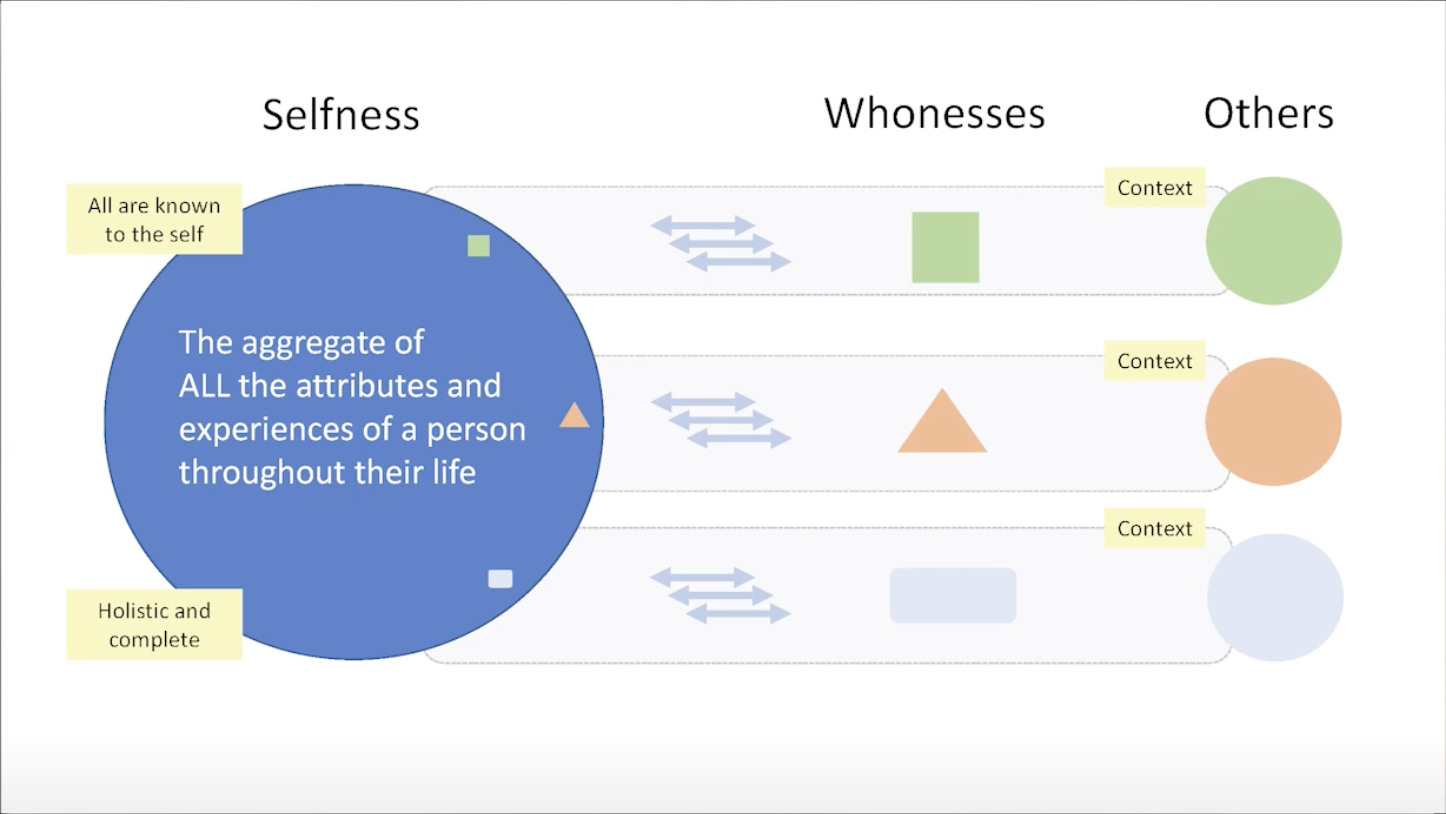
\includegraphics[width=\textwidth]{./images/selfness-and-whoness-larger.png}

\subsection{Open source}

In order to trust that the agent does what we claim, we need transparency which open source can provide. Further this is an ambitious project and we need to nurture the creation of a community of developers help build it.

\subsection{Data Governance}

Once data is shared from the agent to a first-party there are no technical means to constraint what the recipient does with it. No technical means can prevent them from selling it others, for example. Instead, legal means must be employed. Rather than wait for privacy regulations to get strong enough, we propose that first-parties sign a Human Information License to license the user's information under terms that are fair and balanced and respect the user's privacy rights. The contract can be signed by an entity that represents the user to make it effortless for the user.

\subsection{User rights}

[Talk about how even the best privacy legislation is impotent in practice to protect users because they don't require associated technical means to implement them]

\subsection{Enforcement}

Talk here about the need for an entity to audit and enforce compliance with the legal contract]

\subsection{Privacy by design}

\section{Architecture}
In this section we describe a proposed architecture for an identity agent.

\subsection{Agent}

The agent architecture follows a decentralized, layered architecture shown below. We illustrate this architecture by considering a user, Alice, with her own device (e.g. a smart phone) as well as three Other Parties (OPs): a provider's website, a provider's local app, and another user Bob's agent:

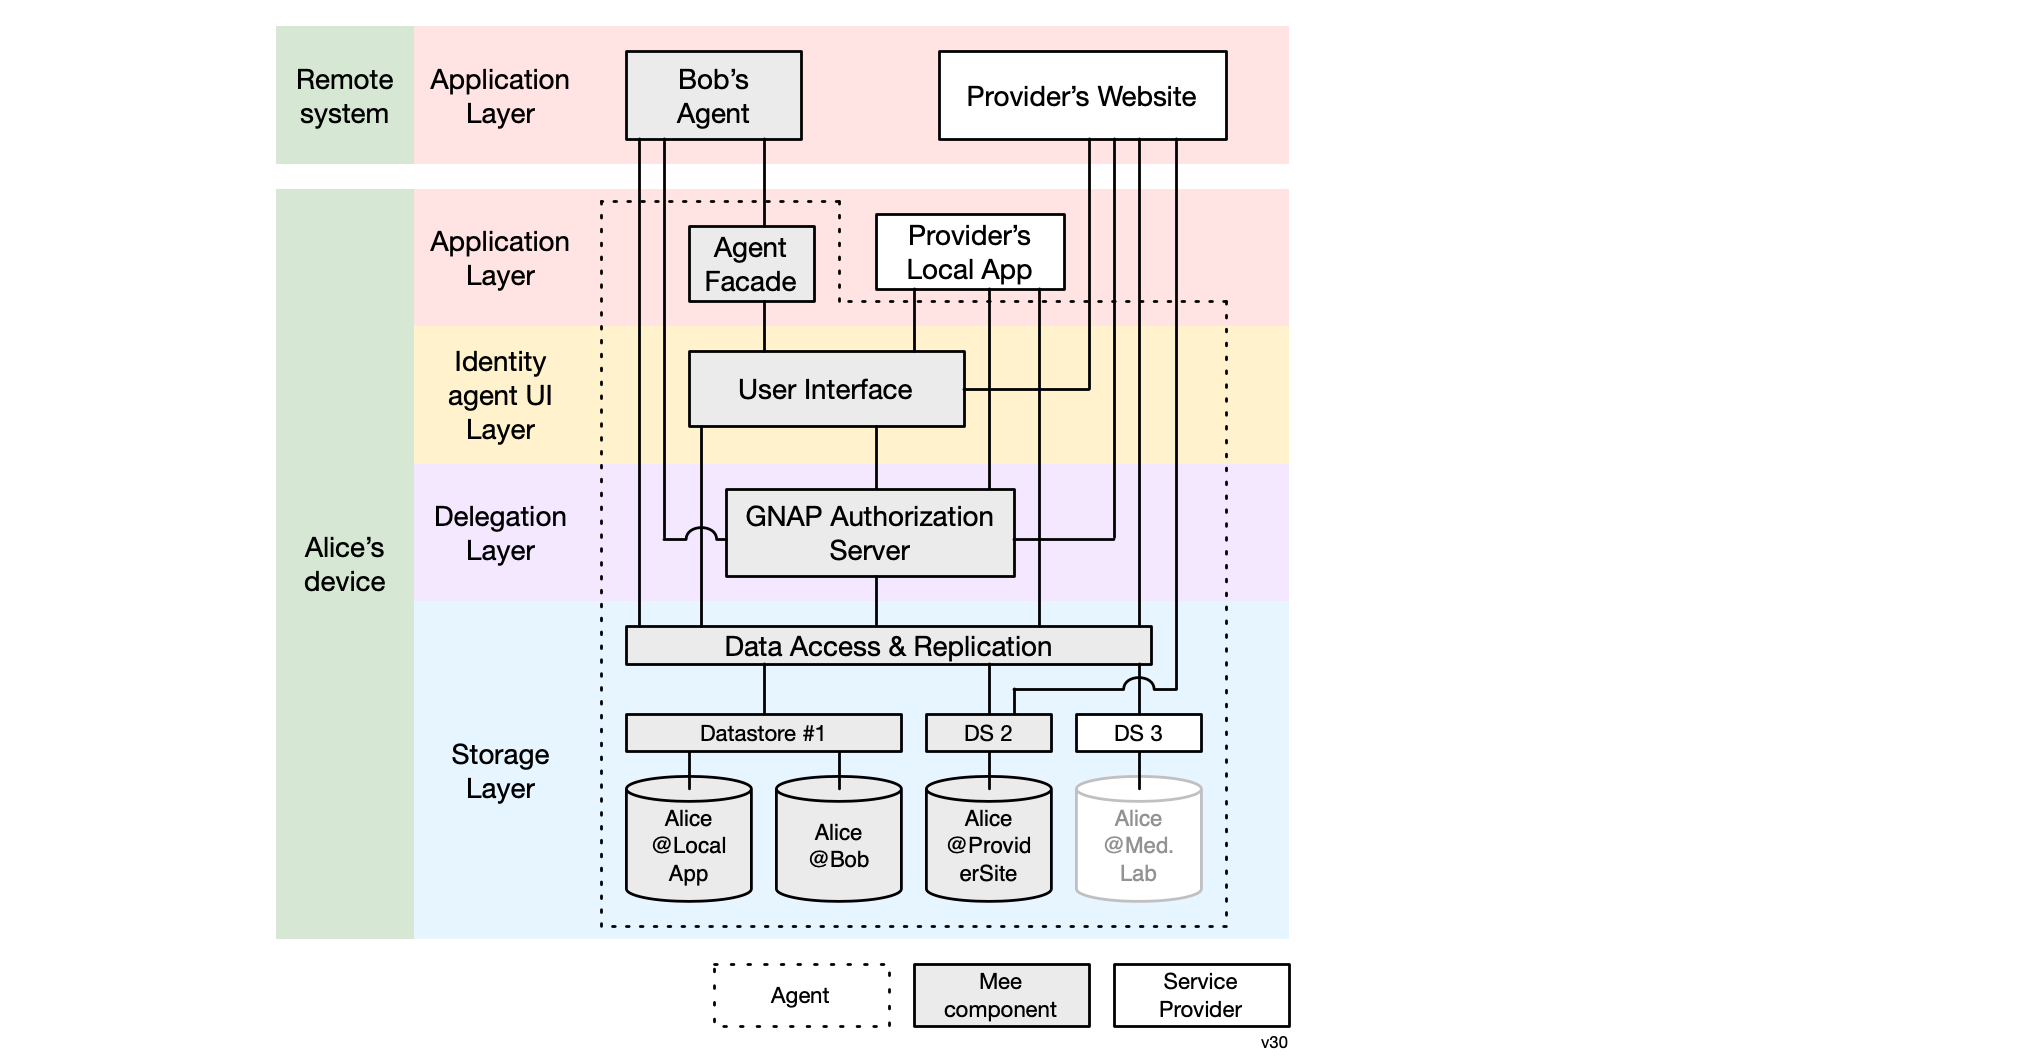
\includegraphics[width=\textwidth]{./images/architecture.png}

\subsubsection{Application layer}

Compatible applications in the application layer may be service provider websites (``Provider's Website" above), other user's agents running on their own devices (``Bob's Agent"), or a service provider's local app running on Alice's device (``Provider's Local App"). Alice's agent appears to other users' agents as an app. The component supporting this on Alice's side is called the Agent Facade.

\subsubsection{Identity agent UI layer}

Alice's identity agent is deployed as an app on Alice's device. The top of layer of the agent is the UI layer that provides Alice with data management features to connect with apps/sites and manage her data. This UI allows her to inspect and in some cases edit each of the partial representations of her in each connection's context(s). 

\subsubsection{Delegation layer}

The delegation layer handles requests for access to data from Alice's agent, local apps, remote apps, and other users' agents. In response to these requests, Alice's authorization server grants or revokes access to data in the context data storage layer. 

\subsubsection{Storage layer}

The data access and replication component provides data access (as controlled by authorization server above it) to the data in each of Alice's contexts. It manages the replication of changes to the data in one of Alice's contexts both (i) between the corresponding app and Alice's agent as well as (ii) among Alice's edge devices (phone, tablet, laptop, etc.).

This layer holds a set of contextualized representations of Alice as defined and created by apps/sites. The diagram above shows three local context data containers on Alice's device and one, the Med Lab app's context data container, which is not replicated on Alice's local device (perhaps because its data set is too large for Alice's device).

\subsection{MeeTalk}

Agents interact with OPs using protocols defined by open standards (e.g. OpenID Connect SIOPv2, etc.). This project is developing a protocol suite called MeeTalk that provides a technical mechanism to respect the agent user's data rights to access, correct (editing), and delete their information held by the OP. An OP must respect these rights in order to become Mee-certified under the terms of the Mee Human Information License. One way to do this is to implement MeeTalk, although we may add support in the future for other protcols that can achieve the same result. We include a discussion of MeeTalk here on the Architecture page because it's implementation mirrors and re-uses certain components of the agent's architecture on the OP side. Shown below is an example of using MeeTalk to communicate between the agent and a provider's website:

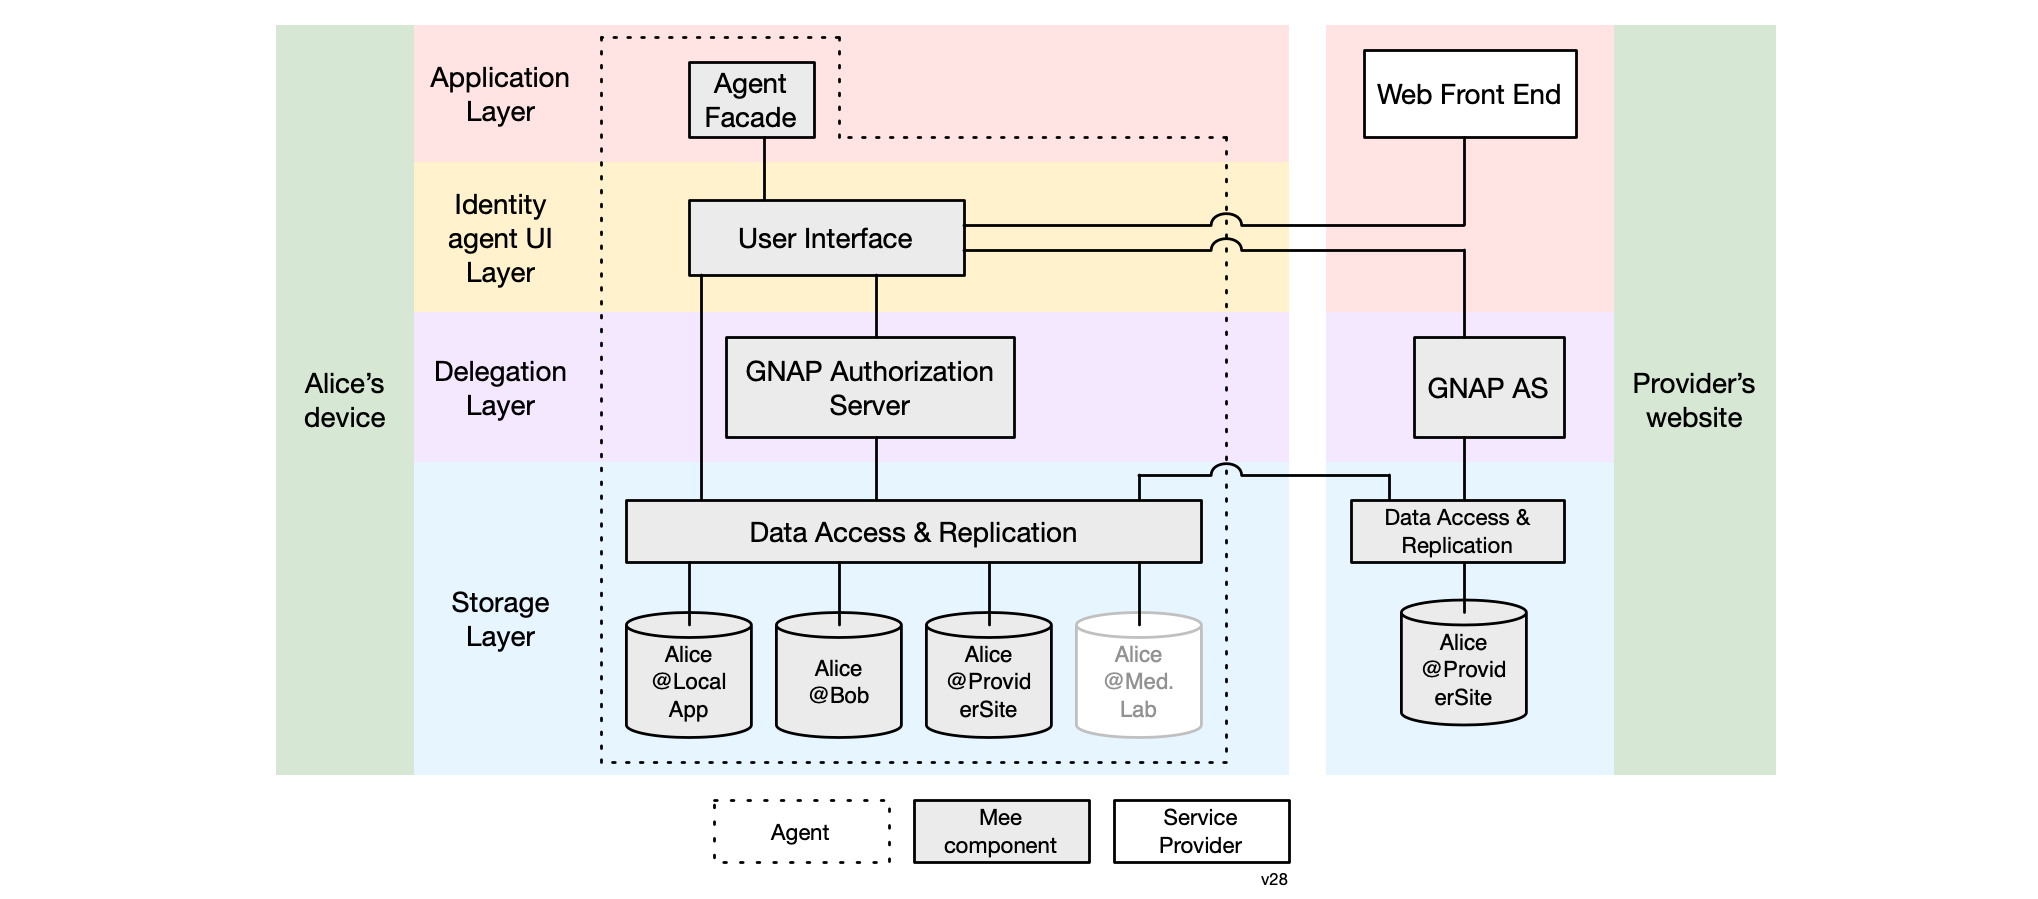
\includegraphics[width=\textwidth]{./images/meetalk.png}
 
    
\bibliographystyle{plain}
\bibliography{mybibliography}


\end{document}  